\section{Das ZAl}
\subsection{Das Zentrale Arbeitslager der Organisation Schmelt}
Der SS-Oberführer und Breslauer\index{o}{Breslau} Polizeipräsident Albrecht Schmelt\index{p}{Schmelt, Albrecht} koordinierte in seiner Position als \glqq Sonderbeauftragter des Reichsführers der SS für fremdvölkischen Arbeitseinsatz in Oberschlesien\grqq, seit 1940 die Zwangsarbeit in Ghettos und Arbeitslagern. Die nach ihm benannte Organisation operierte anfangs nur in Oberschlesien weitete sich jedoch schon bald nach Niederschlesien und ins Sudetenland aus. Es entstanden so genannte Zentrale Arbeitslager (ZAL) in der Nähe von kriegswichtigen Unternehmen wie der WUMAG Görlitz\footnote{Bei einer Wirtschaftsprüfung vom 29. Oktober bis 9. November 1940 wurde die WUMAG zum kriegswichtigen Unternehmen erklärt. StArchD 11693 / 1258 Bild-Chronik III. Das ZAL Görlitz wird in Zusammenhang mit dem Rüstungsbetrieb WUMAG genannt. Vgl. Alfred Konieczny: Die Zwangsarbeit der Juden in Schlesien im Rahmen der Organisation Schmelt, S. 104.}, in denen zumeist die jüdische Bevölkerung Oberschlesiens Zwangsarbeit verrichtete\footnote{Vgl. Martin Weinmann: Das Nationalsozialistische Lagersystem, S. LVIII.}. \glqq Die organisatorische Umsetzung des Zwangsarbeitereinsatzes oblag den Jüdischen Ältestenräten in Oberschlesien, die auf deutsche Verordnung in Sosnowiec zusammengefasst waren [...]\grqq, schreibt Andrea Rudorff\footnote{Andrea Rudorff: Das Lagersystem der Organisation Schmelt in Oberschlesien. S. 159.}. Die Verteilung jüdischer Arbeitskräfte richtete sich nach den Bedarfsmeldungen der Betriebe, anhand derer der Jüdische Ältestenrat der Organisation Schmelt schriftliche Aufforderungen zum Arbeitseinsatz versandt. Die Verteilung jüdischer Arbeitskräfte beruhte auf einer zwischen Schmelt und den jeweiligen Betrieben getroffenen Vereinbarung, die im Sinne strikter Aufwandsminimierung die Löhne und die innere Organisation der Arbeitslager festlegte\footnote{Vgl. Israel Gutman: Enzyklopädie des Holocaust -- Band 2, S. 1070.}. Schmelts\index{p}{Schmelt, Albrecht} Lagerführung stützte sich auf eine Häftlingsselbstverwaltung, die sich bereits in Konzentrationslagern bewährte hatte, und sparte somit an Wachpersonal. Es gab einen Ältesten, einen Krankenbehandler und einen Stenotypisten für je 150 Zwangsarbeiter, genauso wie einen Schuster, einen Schneider und einen Koch samt Küchengehilfen\footnote{Vgl. Martin Weinmann: Das nationalsozialistische Lagersystem (CCP), S. LVIII. Vgl. Alfred Konieczny: Die Zwangsarbeit der Juden in Schlesien im Rahmen der Organisation Schmelt, S. 101.}. Somit genügte ein Wachmann bzw. Hilfspolizist oder Angehöriger des Werkschutzes zur Bewachung von je 40 Gefangenen.
\newline
Der bisherige Erkenntnisstand über das Lagersystem der Organisation Schmelt insgesamt sowie über das ZAL Görlitz im Speziellen ist äußerst unzureichend und beschränkt sich auf wenige Quellen\footnote{Vgl. Andrea Rudorff: Das Lagersystem der Organisation Schmelt in Oberschlesien. S. 159.}.
Das Lager der Organisation Schmelt in Görlitz entstand wahrscheinlich am 26. April 1943\footnote{Entsprechend einer Notiz in der \glqq Chronik zur Geschichte des antifaschistischen Widerstandskampfes\grqq. Nathan Klajman\index{p}{Klajman, Nathan} gibt an, im Mai desselben Jahres in das Lager gekommen zu sein. ZHI 301/2765.} im Biesnitzer Grund. Hinweise, wonach im April 1943 die Häftlinge des ZAL Görlitz nach Kittliztreben (Trzebień, Polen)\index{o}{Kittliztreben} überstellt wurden\footnote{Martin Weinmann: Das nationalsozialistische Lagersystem (CCP), S. 579.} konnten ebenso wenig bestätigt werden wie die Existenz eines \glqq Judenlagers\grqq~innerhalb des Maschinenbaukomplexes der WUMAG (siehe Luftaufnahme S.~\pageref{maschinenbaufoto})\footnote{Nach Ermittlungen von Kurt Wolf aus Löbau, der mir seine Erkenntnisse im Zusammenhang mit dem Schmelt-Lager und dem Außenlager Görlitz zuteil werden ließ.}.
Zeitzeugenberichte aus dem Biesnitzer Lager sind äußerst rar. Die Familie Ecke des benachbarten Bauernhofes hatte während dieser Zeit jedenfalls Zugang zum Lager, um dort die Jauche aus der Latrine abzuschöpfen. Der Bauer Ecke\index{p}{Ecke, Erich} pflegte sogar eine persönliche Beziehung zu einem der Insassen\footnote{Es kam während dessen zu Tauschgeschäften (Leder und Stoffe) zwischen Eckes und dem Gefangenen. Nach der Befreiung des Lagers kam es zu einem Wiedersehen auf dem Hof der Eckes. Laut Aussage von Alfred Ecke.}.~\newline
Der Schmelt-Häftling Nathan Klajman\index{p}{Klajman, Nathan}:
\begin{leftbar}
Im Mai 1943 wurde ich zusammen mit 70 Leuten ins Konzentrationslager nach Görlitz verschleppt. Dort waren 200 Juden. Wir arbeiteten in der Munitionsfabrik, wir wurden unbarmherzig geschlagen. Der Judenälteste Babinger\index{p}{Babinger} war zu uns sehr gut.
Ich blieb dort 10 Monate. Wir bekamen 40 dkg [= 400 Gramm] Brot und Suppe. Die Meister misshandelten uns.\footnote{Nathan Klajman ist in Berlin geboren und durchlebte eine ganze Reihe von Arbeitslagern, darunter Annaberg (auch \glqq Kretschamberg\grqq, heute Cha\l upki, Polen), Graditz (Oberschlesien), bevor er in das KZ-Außenlager Kittlitzstreben (Trzebień, Polen) gebracht wurde. Anfang Februar zwang man ihn und viele andere, einen Todesmarsch über Görlitz nach Zittau anzutreten. Zu Kriegsende befreite man ihn im KZ-Außenlager Zittau (heute: Sieniawka, Polen). ZIH 301/2765.}
\end{leftbar}
Der Schmelt-Häftling Jakob F.\index{p}{F., Jakob}:
\begin{leftbar}
Nach 5--6 Monaten wurde eine Gruppe von 50 Mann, darunter auch ich, [vom ZAL Neukirchen\index{o}{Neukirchen} bei Breslau\index{o}{Breslau}] nach Görlitz abtransportiert. [...] Görlitz war ein kleines Judenlager, ca. 300--350 Juden. Gearbeitet wurde bei der Firma WUMAG -- Waggon- und Maschinenbau -- ein großer Betrieb. [...] Ich mit noch acht Kameraden waren beschäftigt bei Dudel\index{p}{Dudel} als Schachtarbeiter und beim Bau großer Fabrikhallen. Kleidung: Zivil. [...] Bewachung: Wehrmacht. Bei der Arbeit bewacht durch Werkschutzleute des Betriebes Waggonbau. Judenältester: Benjamin R.\index{p}{R., Benjamin} [...] Judenfrauen: 12--13Frauen als Lagerpersonal. [...] Nach 2--3 Monaten wurden die Frauen abtransportiert, wohin weiß ich nicht. Anfang 1944 wurde Görlitz liquidiert und wir kamen ins KZ Kittlitztreben\index{o}{Kittlitztreben} [Trzebień, Polen].\footnote{Der Nachname des Zeugen wurde aus datenschutzrechtlichen Gründen vom Internationalen Suchdienst in Bad Arolsen nicht bekannt gegeben. ISD Sachdokumente M 9 Sakrau, S. 1 (2006).}
\end{leftbar}


\subsection{B}

\glqq Das Schicksal der jüdischen Gefangenen in den Lagern der Organisation Schmelt unterschied sich zum größten Teil nicht von dem aller anderen Insassen von Konzentrationslagern.\grqq, heißt es in der Enzyklopädie des Holocaust\footnote{Israel Gutman (Hrsg.): Enzyklopädie des Holocaust, Band 2, S. 1071.}.
\newline
Nathan Klajman\index{p}{Klajman, Nathan} gab an, zwischen Mai 1943 und März 1944 im ZAL Görlitz inhaftiert gewesen zu sein
\footnote{Nathan Klajman, ZIH 301/2765.}. Anhand der Belegschaftsstatistiken der WUMAG kann keine Belegung mit Schmelt-Häftlingen belegt werden. Offenbar wurden jene Zwangsarbeiter entgegen späterer Statistiken entsprechend ihrer Nationalität, statt vermeintlichen Religionszugehörigkeit verzeichnet\footnote{Zwischen Februar und März 1944 reduziert sich die Zahl der unter \glqq Sonstige\grqq~erfassten Ausländer um 85 Personen. Neben Belgiern, Franzosen, Polen und Russen erscheint die Zeile \glqq Sonstige\grqq~ab September 1944 mit dem handschriftlichen Vermerk \glqq Juden und Häftlinge\grqq. StArchD 11693 / 1258 (Bild-Chronik III).}.
\newline
Bereits Ende 1941 beschloss man im Zusammenhang mit der Endlösung der Judenfrage erstmals die Auflösung der ohnehin zeitlich befristeten ZAL. Die Umsetzung des Beschlusses verschob sich aufgrund erheblicher Einwände seitens der Wehrmacht und des Reichssicherheitshauptamtes, bis Himmler\index{p}{Himmler, Heinrich} 1943 die Auflösung der Lager, in denen die Arbeitskraft der Häftlinge als nicht kriegswichtig angesehen wurde, durchsetzte. Die WUMAG Görlitz befand sich in dieser Zeit in einer starken Abhängigkeit von ausländischen und jüdischen Fachkräften, um die von der Wehrmacht geforderten Rüstungsgüter liefern zu können\footnote{Vgl. Thomas Warkus: Kriegsgefangene und Fremdarbeiter im nationalsozialistischen Deutschland 1939--1945. Das Beispiel Görlitz.}. Es bestand also eine Notwendigkeit möglichst alle Arbeitskräfte zu behalten.
Unter der Führung von Adolf Eichmann\index{p}{Eichmann, Adolf} wurden 28 Lager in Niederschlesien und im Sudetenland -- nach vorheriger \glqq Selektion\grqq~der Häftlinge -- dem KZ Groß-Rosen\index{o}{Groß-Rosen} angegliedert, 20 davon als Außenlager\footnote{15 dieser Lager übergab man der Kommandantur von Auschwitz.}. Häftlinge aus über 125 Lagern wurden auf die Außenlager\footnote{Im folgenden soll nun von \glqq Außenlagern\grqq~oder \glqq Nebenlagern\grqq~gesprochen werden. Im SS-Sprachgebrauch hießen diese Lager im Falle von Männerlagern \glqq Arbeitslager\grqq~(abgekürzt AL) und bei Frauenlagern \glqq Frauenarbeitslager\grqq~(FAL), zum Teil auch \glqq Außenkommandos\grqq. Vgl. Isabell Sprenger: Groß-Rosen, S. 227.} von Groß-Rosen\index{o}{Groß-Rosen} und Auschwitz\index{o}{Auschwitz} verteilt\footnote{Vgl. Alfred Konieczny: Die Zwangsarbeit der Juden in Schlesien im Rahmen der Organisation Schmelt, S. 107.}. Das ZAL in Görlitz muss als eines der letzten Lager, spätestens Mitte 1944, von Groß-Rosen\index{o}{Groß-Rosen} übernommen worden sein.


%\myfigure[lagerluft]{lager0}{Luftbilddatenbank, Ing.-Büro Dr. H.G. Carls.}{Luftaufnahme des Barackenlagers im Biesnitzer Grund vom 30. Mai 1944}{Luftaufnahme des Lagers, 30. Mai 1945}{0}%0.78
\begin{flushleft}
    \setlength{\fboxsep}{0pt}
\begin{figure}
	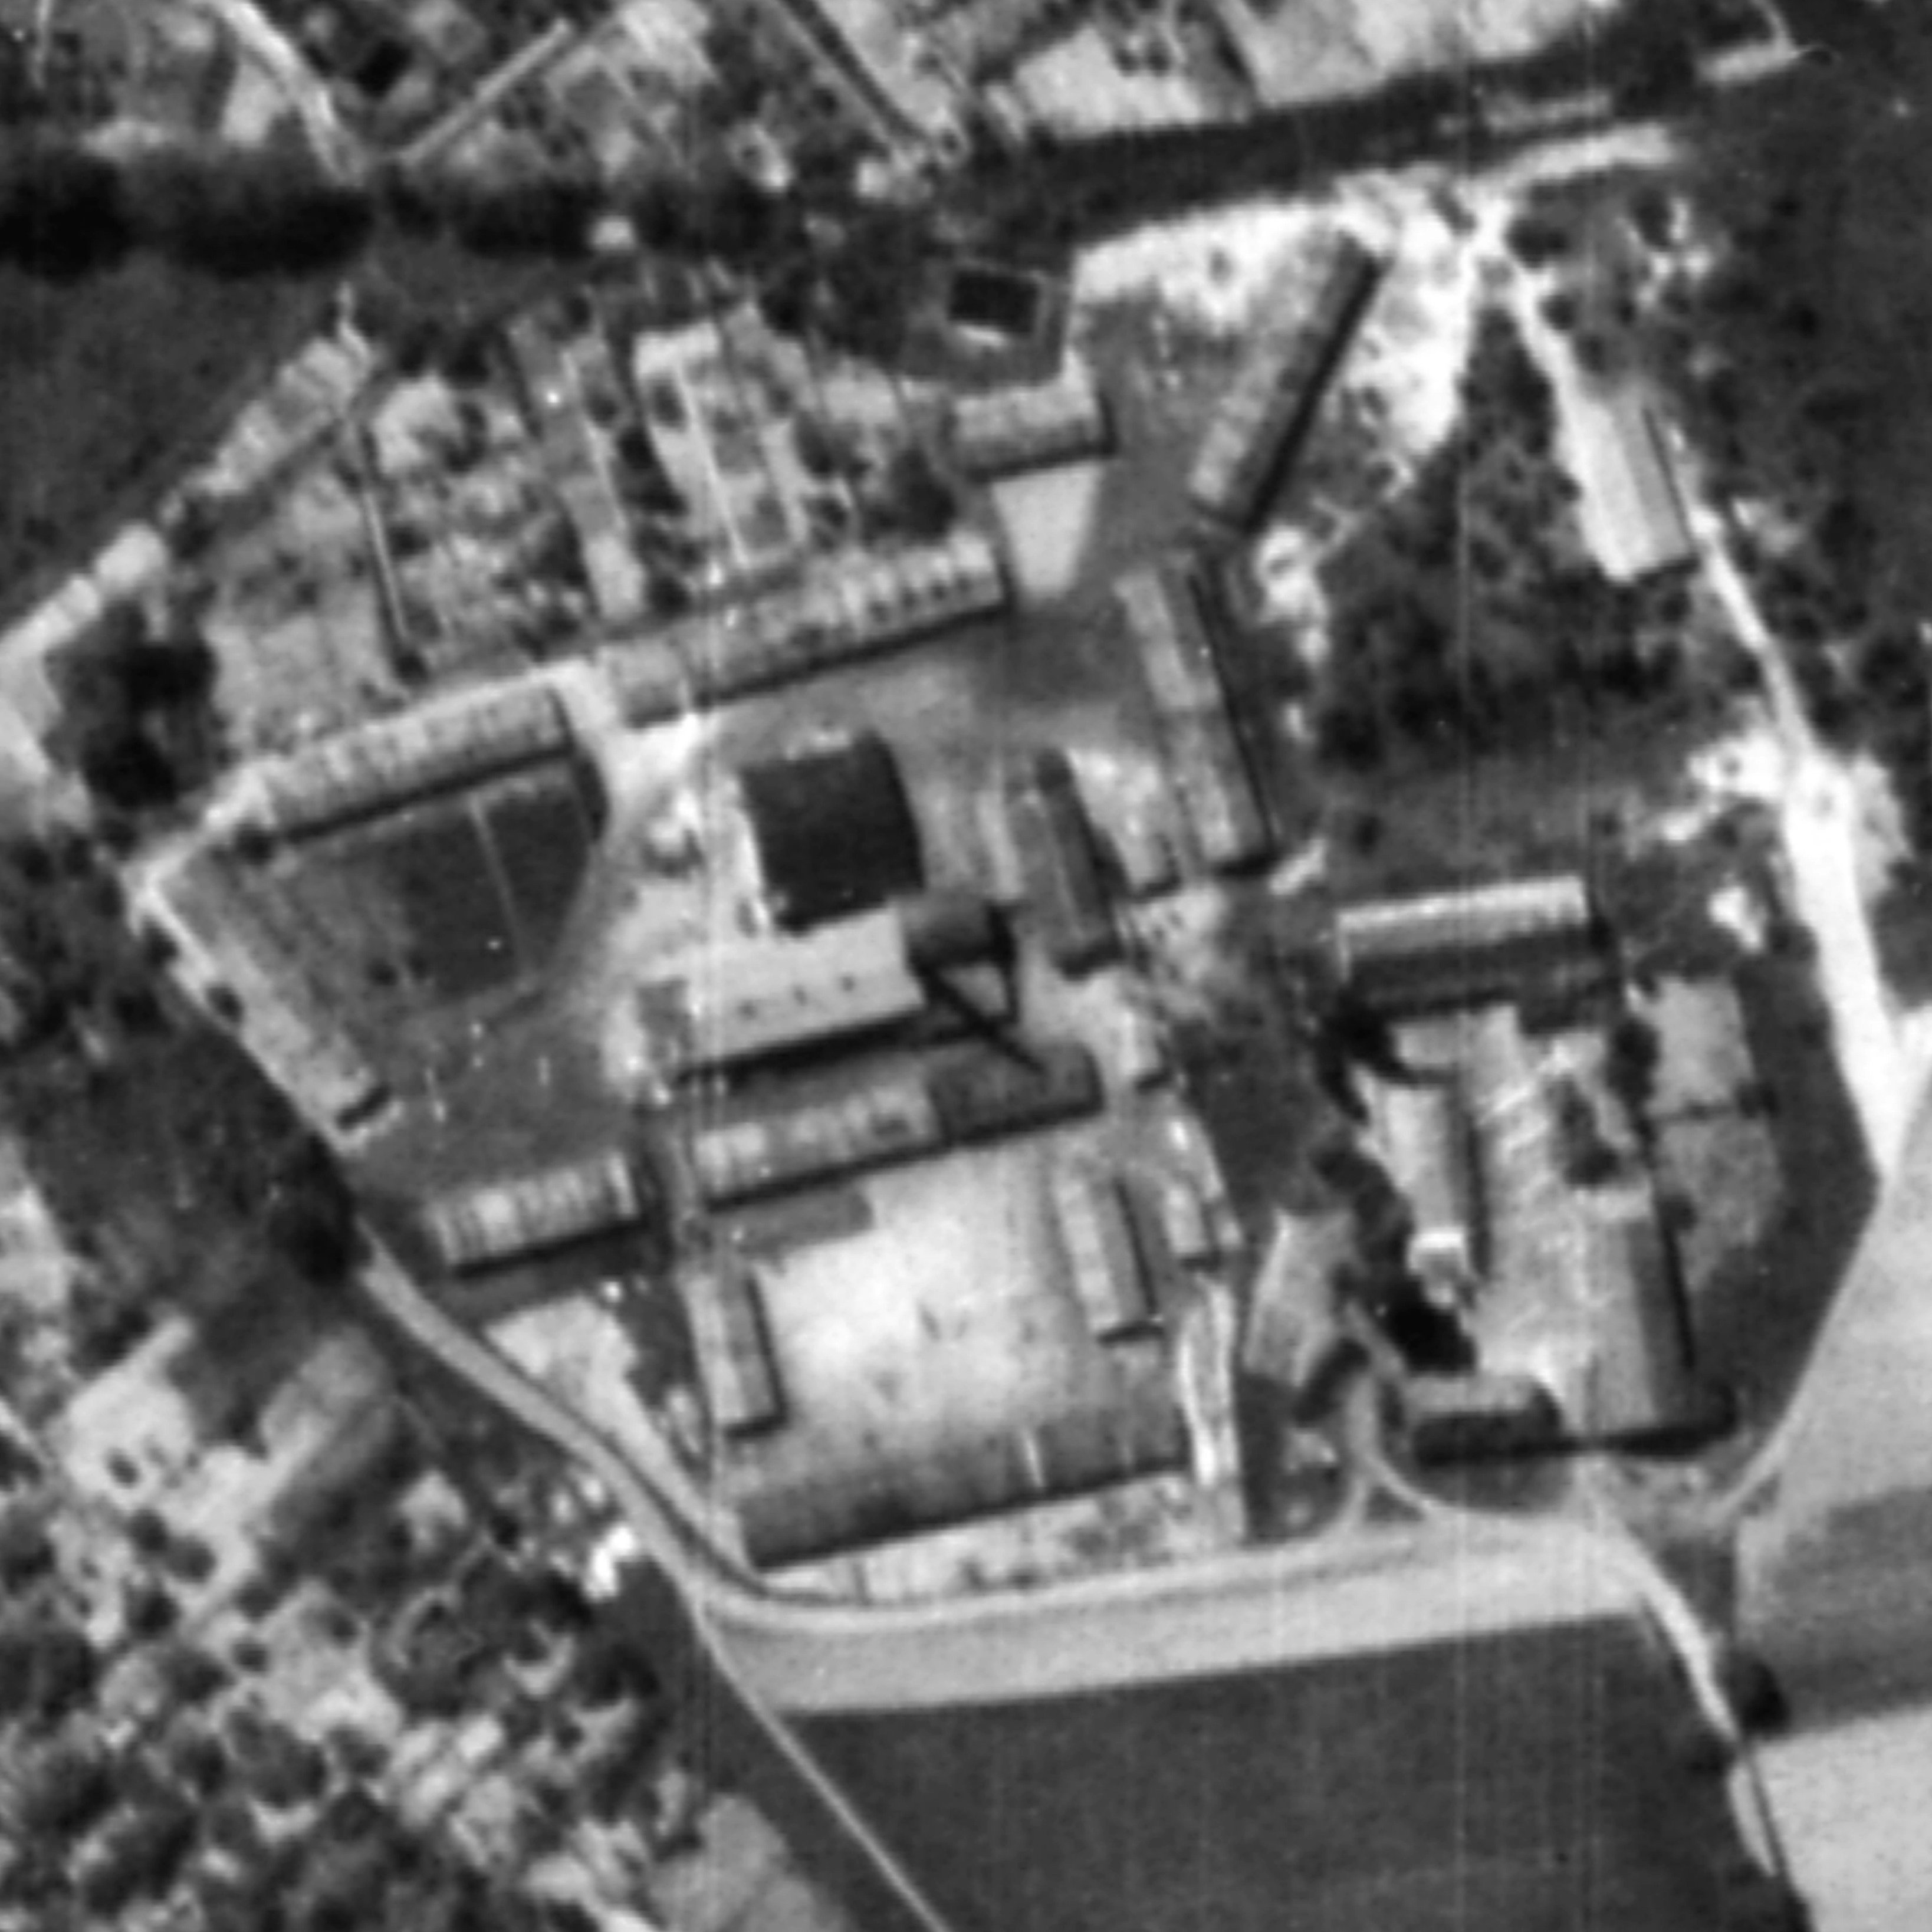
\includegraphics[width=.99\linewidth]{images/lager0.jpg}\fbox{e}
	\caption[Luftaufnahme des Lagers, 30. Mai 1945]{Luftaufnahme des Barackenlagers im Biesnitzer Grund vom 30. Mai 1944. Luftbilddatenbank, Ing.-Büro Dr. H.G. Carls.}
\end{figure}
\end{flushleft}